%%%%%%%%%%%%%%%%%%%%%%%%%%%%%%%%%%%%%%%%%
% Masters/Doctoral Thesis
% LaTeX Template
% Version 2.5 (27/8/17)
%
% This template was downloaded from:
% http://www.LaTeXTemplates.com
%
% Version 2.x major modifications by:
% Vel (vel@latextemplates.com)
%
% This template is based on a template by:
% Steve Gunn (http://users.ecs.soton.ac.uk/srg/softwaretools/document/templates/)
% Sunil Patel (http://www.sunilpatel.co.uk/thesis-template/)
%
% Template license:
% CC BY-NC-SA 3.0 (http://creativecommons.org/licenses/by-nc-sa/3.0/)
%
%%%%%%%%%%%%%%%%%%%%%%%%%%%%%%%%%%%%%%%%%

%----------------------------------------------------------------------------------------
%	PACKAGES AND OTHER DOCUMENT CONFIGURATIONS
%----------------------------------------------------------------------------------------

\documentclass[
11pt, % The default document font size, options: 10pt, 11pt, 12pt
%oneside, % Two side (alternating margins) for binding by default, uncomment to switch to one side
english, % ngerman for German
singlespacing, % Single line spacing, alternatives: onehalfspacing or doublespacing
%draft, % Uncomment to enable draft mode (no pictures, no links, overfull hboxes indicated)
%nolistspacing, % If the document is onehalfspacing or doublespacing, uncomment this to set spacing in lists to single
%liststotoc, % Uncomment to add the list of figures/tables/etc to the table of contents
%toctotoc, % Uncomment to add the main table of contents to the table of contents
%parskip, % Uncomment to add space between paragraphs
%nohyperref, % Uncomment to not load the hyperref package
headsepline, % Uncomment to get a line under the header
%chapterinoneline, % Uncomment to place the chapter title next to the number on one line
%consistentlayout, % Uncomment to change the layout of the declaration, abstract and acknowledgements pages to match the default layout
]{MastersDoctoralThesis} % The class file specifying the document structure

\usepackage[utf8]{inputenc} % Required for inputting international characters
\usepackage[T1]{fontenc} % Output font encoding for international characters

\usepackage{mathpazo} % Use the Palatino font by default
\usepackage{amsmath}
\usepackage{siunitx}
\usepackage{tikz}
\usepackage{minted}

\usepackage[backend=bibtex,style=authoryear,natbib=true]{biblatex} % Use the bibtex backend with the authoryear citation style (which resembles APA)

\addbibresource{biblio.bib} % The filename of the bibliography

\usepackage[autostyle=true]{csquotes} % Required to generate language-dependent quotes in the bibliography

\newcommand{\concat}{\mathbin{\|}}

%----------------------------------------------------------------------------------------
%	MARGIN SETTINGS
%----------------------------------------------------------------------------------------

\geometry{
	paper=a4paper, % Change to letterpaper for US letter
	inner=2.5cm, % Inner margin
	outer=3.8cm, % Outer margin
	bindingoffset=.5cm, % Binding offset
	top=1.5cm, % Top margin
	bottom=1.5cm, % Bottom margin
	%showframe, % Uncomment to show how the type block is set on the page
}

%----------------------------------------------------------------------------------------
%	THESIS INFORMATION
%----------------------------------------------------------------------------------------

\thesistitle{Flexible Channels: Preventing Metadata Leakage in Communication over Public Channels} % Your thesis title, this is used in the title and abstract, print it elsewhere with \ttitle
\supervisor{Prof. Hidehiko \textsc{Masuhara}} % Your supervisor's name, this is used in the title page, print it elsewhere with \supname
\examiner{} % Your examiner's name, this is not currently used anywhere in the template, print it elsewhere with \examname
\degree{Master of Science} % Your degree name, this is used in the title page and abstract, print it elsewhere with \degreename
\author{Jacob \textsc{Lindahl}} % Your name, this is used in the title page and abstract, print it elsewhere with \authorname
\addresses{} % Your address, this is not currently used anywhere in the template, print it elsewhere with \addressname
\studentnum{21M38053}
\subject{Mathematics and Computing Science} % Your subject area, this is not currently used anywhere in the template, print it elsewhere with \subjectname
\keywords{} % Keywords for your thesis, this is not currently used anywhere in the template, print it elsewhere with \keywordnames
\university{\href{http://www.titech.ac.jp}{Tokyo Institute of Technology}} % Your university's name and URL, this is used in the title page and abstract, print it elsewhere with \univname
\department{\href{https://educ.titech.ac.jp/is/}{Department of Mathematical and Computing Science}} % Your department's name and URL, this is used in the title page and abstract, print it elsewhere with \deptname
\group{\href{https://prg.is.titech.ac.jp/}{Programming Research Group}} % Your research group's name and URL, this is used in the title page, print it elsewhere with \groupname
\faculty{\href{https://www.titech.ac.jp/about/organization/schools/organization04.html}{School of Computing}} % Your faculty's name and URL, this is used in the title page and abstract, print it elsewhere with \facname

\AtBeginDocument{
\hypersetup{pdftitle=\ttitle} % Set the PDF's title to your title
\hypersetup{pdfauthor=\authorname} % Set the PDF's author to your name
\hypersetup{pdfkeywords=\keywordnames} % Set the PDF's keywords to your keywords
}

\begin{document}

\frontmatter % Use roman page numbering style (i, ii, iii, iv...) for the pre-content pages

\pagestyle{plain} % Default to the plain heading style until the thesis style is called for the body content

%----------------------------------------------------------------------------------------
%	TITLE PAGE
%----------------------------------------------------------------------------------------

\begin{titlepage}
\begin{center}

\includegraphics[scale=0.3]{Figures/titech.pdf} \\[0.1cm]
\vspace*{.01\textheight}
{\scshape\LARGE \univname\par}\vspace{1.5cm} % University name
\textsc{\Large Master Thesis}\\[0.5cm] % Thesis type

\HRule \\[0.4cm] % Horizontal line
{\huge \bfseries \ttitle\par}\vspace{0.4cm} % Thesis title
\HRule \\[1.5cm] % Horizontal line

\begin{minipage}[t]{0.4\textwidth}
\begin{flushleft} \large
\emph{Author:}\\
\href{https://prg.is.titech.ac.jp/people/jacob-lindahl/}{\authorname}\\[0.3cm] % Author name - remove the \href bracket to remove the link
\emph{Student Number:}\\
\textsc{\studentnumname}
\end{flushleft}
\end{minipage}
\begin{minipage}[t]{0.4\textwidth}
\begin{flushright} \large
\emph{Supervisor:} \\
\href{http://prg.is.titech.ac.jp/people/masuhara/}{\supname} % Supervisor name - remove the \href bracket to remove the link
\end{flushright}
\end{minipage}\\[3cm]

\vfill

\large \textit{A thesis submitted in fulfillment of the requirements\\ for the degree of \degreename}\\[0.3cm] % University requirement text
\textit{in the}\\[0.4cm]
\groupname\\\deptname\\[2cm] % Research group name and department name

\vfill

{\large \today}\\[4cm] % Date
%\includegraphics{Logo} % University/department logo - uncomment to place it

\vfill
\end{center}
\end{titlepage}

%----------------------------------------------------------------------------------------
%	DECLARATION PAGE
%----------------------------------------------------------------------------------------

% \begin{declaration}
% \addchaptertocentry{\authorshipname} % Add the declaration to the table of contents
% \noindent I, \authorname, declare that this thesis titled, \enquote{\ttitle} and the work presented in it are my own. I confirm that:

% \begin{itemize}
% \item This work was done wholly or mainly while in candidature for a research degree at this University.
% \item Where any part of this thesis has previously been submitted for a degree or any other qualification at this University or any other institution, this has been clearly stated.
% \item Where I have consulted the published work of others, this is always clearly attributed.
% \item Where I have quoted from the work of others, the source is always given. With the exception of such quotations, this thesis is entirely my own work.
% \item I have acknowledged all main sources of help.
% \item Where the thesis is based on work done by myself jointly with others, I have made clear exactly what was done by others and what I have contributed myself.\\
% \end{itemize}

% \noindent Signed:\\
% \rule[0.5em]{25em}{0.5pt} % This prints a line for the signature

% \noindent Date:\\
% \rule[0.5em]{25em}{0.5pt} % This prints a line to write the date
% \end{declaration}

% \cleardoublepage

%----------------------------------------------------------------------------------------
%	QUOTATION PAGE
%----------------------------------------------------------------------------------------

\vspace*{0.2\textheight}

\noindent\enquote{\itshape And so by doing just acts we become just, and by doing acts of temperance and courage we become temperate and courageous.}\bigbreak

\hfill Aristotle, \textit{Nicomachean Ethics}

%----------------------------------------------------------------------------------------
%	ABSTRACT PAGE
%----------------------------------------------------------------------------------------

\begin{abstract}
% \addchaptertocentry{\abstractname} % Add the abstract to the table of contents
Public blockchain ledgers are, at first glance, antithetical to privacy: all data are recorded permanently and publicly. While this is necessary, in many cases, to trustlessly verify the execution of the virtual machine, by the same token, blockchains are not often used to directly store sensitive information. However, popular blockchains do provide data distribution (data availability), historical execution auditability, and data accessibility that have interesting implications for encrypted messaging. The disadvantages for using a blockchain as the underlying middleman for an encrypted messaging system are clear and numerous: cost, privacy, efficiency, etc. We present a protocol that attempts to mitigate these issues while taking advantage of the unique mechanisms that blockchains do provide, and provide recommendations for similar projects.
\end{abstract}

%----------------------------------------------------------------------------------------
%	ACKNOWLEDGEMENTS
%----------------------------------------------------------------------------------------

\begin{acknowledgements}
% \addchaptertocentry{\acknowledgementname} % Add the acknowledgements to the table of contents
The most heartfelt thanks I give to my supervisor, Prof. Hidehiko Masuhara, for his guidance, patience, and support. I am grateful for the opportunity to work with him and learn from him.

To my friends and family for their support and encouragement, I thank you.

To the members of the Programming Research Group for their feedback and support, I am grateful.

To my Lord and Savior, Jesus Christ, for His grace and mercy, I am awestruck.
\end{acknowledgements}

%----------------------------------------------------------------------------------------
%	LIST OF CONTENTS/FIGURES/TABLES PAGES
%----------------------------------------------------------------------------------------

\tableofcontents % Prints the main table of contents

\listoffigures % Prints the list of figures

% \listoftables % Prints the list of tables

%----------------------------------------------------------------------------------------
%	ABBREVIATIONS
%----------------------------------------------------------------------------------------

\begin{abbreviations}{ll} % Include a list of abbreviations (a table of two columns)

\textbf{GWei} & \textbf{G}iga \textbf{Wei} ($10^9$ units of the native Ethereum cryptocurrency)\\
\textbf{HMAC} & \textbf{H}ash-based \textbf{M}essage \textbf{A}uthentication \textbf{C}ode\\
\textbf{HMAC-SHA3-512} & \textbf{HMAC} using the \textbf{SHA3-512} hash function\\
\textbf{PKI} & \textbf{P}ublic \textbf{K}ey \textbf{I}nfrastructure\\
\textbf{RPC} & \textbf{R}emote \textbf{P}rocedure \textbf{C}all\\
\textbf{SHA} & \textbf{S}ecure \textbf{H}ash \textbf{A}lgorithm\\
\textbf{TLS} & \textbf{T}ransport \textbf{L}ayer \textbf{S}ecurity\\
\textbf{URI} & \textbf{U}niform \textbf{R}esource \textbf{I}dentifier\\
\textbf{zk-SNARK} & \textbf{Z}ero-\textbf{K}nowledge \textbf{S}uccinct \textbf{N}on-Interactive \textbf{Ar}gument of \textbf{K}nowledge\\
\textbf{ZKP} & \textbf{Z}ero-\textbf{K}nowledge \textbf{P}roof\\

\end{abbreviations}

%----------------------------------------------------------------------------------------
%	PHYSICAL CONSTANTS/OTHER DEFINITIONS
%----------------------------------------------------------------------------------------

% \begin{constants}{lr@{${}={}$}l} % The list of physical constants is a three column table

% % The \SI{}{} command is provided by the siunitx package, see its documentation for instructions on how to use it

% Speed of Light & $c_{0}$ & \SI{2.99792458e8}{\meter\per\second} (exact)\\
% %Constant Name & $Symbol$ & $Constant Value$ with units\\

% \end{constants}

%----------------------------------------------------------------------------------------
%	SYMBOLS
%----------------------------------------------------------------------------------------

% \begin{symbols}{lll} % Include a list of Symbols (a three column table)

% $a$ & distance & \si{\meter} \\
% $P$ & power & \si{\watt} (\si{\joule\per\second}) \\
% %Symbol & Name & Unit \\

% \addlinespace % Gap to separate the Roman symbols from the Greek

% $\omega$ & angular frequency & \si{\radian} \\

% \end{symbols}

%----------------------------------------------------------------------------------------
%	DEDICATION
%----------------------------------------------------------------------------------------

\dedicatory{For Aniyah}

%----------------------------------------------------------------------------------------
%	THESIS CONTENT - CHAPTERS
%----------------------------------------------------------------------------------------

\mainmatter % Begin numeric (1,2,3...) page numbering

\pagestyle{thesis} % Return the page headers back to the "thesis" style

% Include the chapters of the thesis as separate files from the Chapters folder
% Uncomment the lines as you write the chapters

\chapter{Introduction}

\label{Introduction}

\section{Motivation}\label{motivation}

The privacy of digital communications is a critical issue in the Internet age. The Snowden revelations \parencite{greenwald_nsa_2013} have shown that world powers are actively monitoring and collecting data on their citizens. This emphasizes the need for secure communication channels that are resistant to surveillance.

The most popular messaging applications today, such as WhatsApp, Signal, and Telegram, claim to be end-to-end encrypted. Even if so, these applications still have access to metadata about conversations, such as who is talking to whom, when, and how often. This metadata can reveal a lot about a person's social network, habits, and interests, even if only to the platform being used.\footnote{This, of course, become an irrelevant qualifier when governments apply legal pressure to the platforms in question.} In some cases, metadata can be even more revealing than the content of the messages themselves.

Furthermore, the claims of these applications can be misleading. Telegram is an application popularly suggested during discussions of private or encrypted messaging \parencite{collins_best_2022, key_best_2024} and has striking adoption, both within and without of purportedly ``privacy-conscious'' communities. Its encryption protocol \parencite{telegram_mtproto_2021}, though bespoke, has seen favorable reviews \parencite{miculan_automated_2023}. However, it is commonly overlooked that encryption on Telegram is an opt-in feature, requiring users to start a ``Secret Chat'' in order to benefit from the encryption. This is not the default behavior of the application.

\bigskip

Only a few years prior to Snowden, a new contender for censorship-resistance made its appearance: Satoshi Nakamoto published the Bitcoin whitepaper \parencite{nakamoto_bitcoin_2008}, which introduced the concept of a decentralized, trustless, and censorship-resistant currency on a broad scale. The potential of this technology rapidly expanded to include the trustless execution of general-purpose applications, notably in the form of smart contracts on the Ethereum blockchain \parencite{buterin_ethereum_2014}. While blockchain platforms such as these are widely regarded as censorship-resistant, public ledgers are eponymously antipodean to privacy insofar as their contents and execution are intrinsically revealed. Thus, an ``anti-surveillance'' public-ledger blockchain protocol is almost a contradiction in terms: decentralization, and consequently censorship-resistance, is verily achieved by ``surveillance'' of the network by the public.

Although there have been a few forays into \emph{privacy-first} public-ledger cryptocurrency platforms (\cite[CryptoNote:][]{saberhagen_cryptonote_2013}; \cite[Zerocash:][]{sasson_zerocash_2014}), they have not achieved level of adoption of Bitcoin and Ethereum. Additionally, projects like Monero (CryptoNote derivative implementation) and Zcash (the active successor to Zerocash) are not general-purpose virtual machines like Ethereum, targeting only the peer-to-peer medium-of-exchange use case.

Mina Protocol implements a general-purpose virtual machine by using recursive zero-knowledge proofs to compress the blockchain to a constant size proof-of-execution; the state root is included in the proof. \parencite{bonneau_mina_2020} In order to prove state transitions, therefore, the state must be obtained from a source external to the actual blockchain---a data availability layer. While the data could be sourced elsewhere (e.g. directly from the user interacting with an application), for the purposes of a messaging system, whose raison d'\^{e}tre data transmission from one party to another, the data availability infrastructure is not an improvement over the relatively simpler approach of a platform like Ethereum.

\bigskip

Decentralized blockchain platforms have many features that would be valuable in a private messenger: high availability, trustless security, and censorship-resistance. However, they also are non-ideal for a variety of reasons: speed, cost, and inherent tracability, implying ease of deanonymization. We largely do not attempt to address the first two disadvantages, since they are fundamental to the underlying blockchain, the judicious choice of which can be some mitigation. We attempt to combine some fundamental traditional cryptographic techniques with the modern blockchain technology to create a privacy-focused messaging protocol that is resistant to surveillance and censorship by using a blockchain protocol (or other infrastructure with similar properties) as the exclusive intermediary/distribution mechanism. While many of the techniques we use are not new, the combination of them in this context is novel.

We call this protocol \textbf{Flexible Channels}.

\section{Goals}\label{goals}

The goal of Flexible Channels is to build upon the work of previous protocols to hide even more metadata about conversations. In particular, we will hide the following information, in addition to hiding of the payload itself:

\begin{itemize}
\item
  Sender's identity.
\item
  Sender's location (geographical and network).
\item
  Timestamp of transmission.
\item
  Receiver's identity.
\item
  Receiver's location (geographical and network).
\item
  Timestamp of receipt.
\item
  Payload size.
\item
  Conversation history.
\end{itemize}

However, privacy of these data is not sufficient to make a usable protocol. Therefore, we will also aim to fulfill the following properties that make the protocol usable:

\begin{itemize}
\item
  Users can easily use the service across multiple devices, including message synchronization.
\item
  Group messaging is efficient and scalable.
\item
  The service is inexpensive to run as a server and as a user/client.
\end{itemize}

\chapter{Proposal}\label{Proposal}

\section{Protocol}\label{protocol}

The key insights of this paper are the channel and sequence hash constructions.

A channel is a total-ordered stream of messages. It consists of membership list (one or more members of a group) and a shared secret (derivable by Diffie-Hellman or any other method of establishing a shared secret). \parencite{diffie_new_1976}

A channel has a deterministic sequence hash generator. Hashing the fields of the channel, together with a nonce, produces a ``sequence hash.'' This sequence hash can only be recreated by parties privy to the channel's shared secret, yet it does not reveal the shared secret. The sequence hash serves as the identifying key of a message sent to the message repository.

The message repository is a simple construct, consisting of a key-value store from which anyone can read, and to which anyone can write. The only restriction is that existing keys cannot be overwritten. The public nature of the message repository is critical to ensuring the efficiency of group messaging as well as ensuring that a user accessing the system from multiple different terminals is easily able to retrieve previous messages.

Using a series of abstractions, the channel construct can be composed in a number of different ways, supporting $1 \leftrightarrow 1$, $1 \leftrightarrow N$, and $N \leftrightarrow N$ messaging.

Of particular interest is $N \leftrightarrow N$ messaging. If all members of a particular group share the same secret, they can all generate the same sequence of hashes, and decrypt all of the messages in the channel. This allows for posting a single message, encrypted with the shared secret, to the public message repository, and all of the members of the group will be able to read it, regardless of the number of members in the group. Thus, we have $O(1)$ space complexity for broadcast transmissions.

\begin{figure}[h]
    \centering
    \begin{tikzpicture}[
        node distance=1.5cm,
        description/.style={align=left},
        message/.style={rectangle,draw,solid,fill=gray!30,minimum width=30mm,minimum height=8mm},
        private/.style={rectangle,draw,solid,fill=gray!30,minimum width=12mm,minimum height=8mm},
        public/.style={rectangle,draw,solid,fill=white,minimum width=12mm,minimum height=8mm},
        user/.style={rectangle,draw,dotted,fill=gray!10,inner sep=10pt},
        enveloped/.style={rectangle,fill=white,draw,solid,double=gray!10,double distance=.5mm},
        service/.style={rectangle,draw=black,dotted,rounded corners=2em,minimum width=4cm,minimum height=2cm}
    ]

    % Add legend
    \node[description] (legend) {
        \begin{tabular}{l l}
            \raisebox{-1ex}{\tikz\node[private,minimum width=8mm] {};} & Non-public data \\[0.5ex]
            \raisebox{-1ex}{\tikz\node[public,minimum width=8mm] {};} & (Eventually) public data
        \end{tabular}
    };

    \node[user] (user) at ($(legend)+(0,-7.5)$) {
        \begin{tikzpicture}[node distance=1cm]
            \node[message] (message) {$m$};

            \node[private] (chunk1) at ($(message)+(-1,-2)$) {$m_1$};
            \node[private] (chunk2) at ($(message)+(1,-2)$) {$m_2$};
            \node at ($(chunk2)+(1.5,0)$) {$\cdots$};
            \draw[->,solid] (message) -- (chunk1);
            \draw[->,solid] (message) -- (chunk2) node[midway,right] {\textit{Chunking}};

            \node[private] (index) at ($(chunk1)+(-4.5,0)$) {$n$};
            \node[private] (identifier) at ($(index)+(+2,0)$) {$i_{\{S,R\}}$};
            \node[private] (key) at ($(identifier)+(0,2)$) {$k_{\{S,R\}}$};

            \node[public] (encrypted1) at ($(chunk1)+(0,-2)$) {$c^n$};
            \draw[->,solid] (chunk1) -- (encrypted1) node[midway,right] {\textit{Encryption}};
            \draw[->,solid] (key.south east) -- (encrypted1);
            \node at ($(encrypted1)+(1.5,0)$) {$\cdots$};

            \node[public] (hash) at ($(index)+(0,-2)$) {$h^n$};
            \draw[->,solid] (index) -- (hash) node[midway,left] {$H(i_{\{S,R\}}, n)$};
            \draw[->,solid] (identifier) -- (hash);
            \draw[->,solid] (key) -- (identifier) node[midway,left] {$H(k_{\{S,R\}}, v_S \concat v_R)$};

            \node[public] (proof) at ($(hash)+(2,-2)$) {$\pi^n$};
            \draw[->,solid] ($(key.south west)!0.85!(key.south east)$) .. controls +(1.4,-2) and +(0,1) .. (proof);
            \draw[->,solid] (hash) -- (proof) node[midway,left=5mm] {\textit{Proof generation}};
            \draw[->,solid] (encrypted1) -- (proof);

            \node[service] (network) at ($(proof)+(+5,-1)$) {Proxy network};

            \node[enveloped] (onionpayload) at ($(proof)+(0,-2)$) {$(h^n, c^n, \pi^n)$};
            \draw[->,solid] (hash) -- (onionpayload);
            \draw[->,solid] (proof) -- (onionpayload) node[midway,left=5mm] {\textit{Routing encryption}};
            \draw[->,solid] (encrypted1) -- (onionpayload);
            \draw[->,solid] (network.west) .. controls +(-2,0) .. ($(onionpayload.north)+(.5,0)$);

            \draw[->,solid] (onionpayload) .. controls +(0,-2) and +(-1,-2) .. (network) node[midway,right,yshift=-3mm] {\textit{Publish}};

            \node[above right] at (current bounding box.north west) {User};
        \end{tikzpicture}
    };

    \end{tikzpicture}
    \caption{User actions: Message chunking, encryption, sequence hash generation, proving, and proxy routing.}
    \label{fig:message_preparation}
\end{figure}

\subsection{Extensions}\label{extensions}

We propose a number of extensions to the protocol to enhance its usability and privacy:

\begin{itemize}
\item
    \hyperref[garbage-messages]{\textbf{Garbage messages:}} A user can send messages to a channel that are indistinguishable from real messages. This extension is useful for obfuscating the metadata of a user's communications. It is recommended that garbage messages be sent at a Poisson-distributed frequency.
\item
    \hyperref[payload-size]{\textbf{Payload size manipulation:}} The protocol enforces a regulated size for all messages. This extension is useful for obfuscating the metadata of a user's communications by reducing the information that can be gleaned from the size of the payload.
\item
    \hyperref[message-notifications]{\textbf{Message notifications:}} A user can download a single payload which can be analyzed to determine with high probability whether any messages relevant to the user have been posted to the message repository. This extension has an $O(n)$ space complexity, where $n$ is the number of messages sent to the message repository.
\item
    \hyperref[proxies]{\textbf{Proxies:}} A user can send messages to a proxy service, which will then forward the messages to the message repository. This extension is useful for obfuscating the network activity of a user's communications by hiding the user's IP address from the message repository. If the message repository is hosted on a blockchain, this extension is also useful for concealing the user's blockchain identity, since all activity will be initiated by the proxy instead.
\item
    \hyperref[dandelion-style-routing]{\textbf{Dandelion-style routing:}} A user can send messages to the message repository through a series of hops, making it difficult for an observer to determine the origin of the message. This extension is useful for reducing the likelihood that encountering a rogue proxy will compromise the user's privacy.
\end{itemize}

\section{Channels}\label{channels}

Consider a channel with members Sender Steve and Receiver Robin $\mathcal{C}_{\{S,R\}}$, where the public keys $v_S$ and $v_R$ are mutually known. Using Diffie-Hellman or any other method of establishing a shared secret, Steve and Robin can establish a shared secret $k_{\{S,R\}} = \operatorname{Diffie-Hellman}(S, R)$. In combination with other, optional, static metadata, a similarly secret channel identifier $i_{\{S,R\}}$ can be derived. An example of this process is demonstrated below:

$$ i_{\{S,R\}} = H(k_{\{S,R\}}, v_S \concat v_R) $$

where $H$ is a keyed cryptographic hash function (such as HMAC-SHA3-512).

The channel identifier $i_{\{S,R\}}$ is used to identify the channel $\mathcal{C}_{\{S,R\}}$. However, this identifier should not be publicized because it can be used to derive the sequence hashes for the channel before they have been posted to a public message repository. \hyperref[ensuring-proxy-honesty]{Additions to the protocol} relieve the need to keep individual sequence hashes secret, however, revealing a channel identifier would make it possible to generate all sequence hashes for a channel, proving that they are linked.

\section{Generating sequence hashes}\label{generating-sequence-hashes}

Once a channel has been established, the sender and receiver can generate a sequence hash $h_{\{S,R\}}^n$ for the $n$th message in the channel. This sequence hash is used to identify the message in the message repository. The sequence hash is generated as follows:

$$ h_{\{S,R\}}^n = H(i_{\{S,R\}}, n) $$

where $n$ is the sequence number of the message.

\section{Posting and reading messages}\label{posting-and-reading-messages}

Once a sequence hash has been generated, the sender can post a payload $(h_{\{S,R\}}^n, c^n)$ to the message repository, where $c^n$ is the ciphertext of the $n$th message, encrypted with the shared secret $k_{\{S,R\}}$. Once the message has posted, Receiver Robin, knowing the shared secret $k_{\{S,R\}}$ and the index of last message he saw $n-1$, can find the message keyed by $h_{\{S,R\}}^n$ in the message repository, and decrypt it.

\section{Group abstractions}\label{group-abstractions}

When multiple actors have read and write access to a channel by virtue of knowing the channel shared secret, how do they synchronize which channel member is entitled to use which sequence numbers?

As long as all member of a channel have full knowledge of the other members of the channel, this is a trivial problem to solve. The protocol simply defines a deterministic sort order according to which the channel members' respective identifiers are ordered $A$. Then, the $i$th message sent by Steve uses sequence number $i \lvert A \rvert + \operatorname{indexof}(A, S)$. This ensures that each channel member has a predefined set of sequence numbers assigned to them which all other channel members know. This formulation also prevents the race condition where two different members from attempting to use a nonce simultaneously.

However, the downside to this approach is that it requires observers of the channel to check for $O(n)$ message receipts where $n$ is the number of members in the channel. In the case of large channels, this can cause excessive network activity even when the channel itself has low activity. This can be somewhat mitigated with \hyperref[message-notifications]{the message notification extension described below}.

\section{Garbage messages}\label{garbage-messages}

While any party without knowledge of the channel's shared secret is incapable of decrypting the messages within a channel, if a channel member's network activity is being monitored or if the message repository that a channel is using has very low traffic, it becomes possible to deduce increasingly detailed metadata about channel participants even if the contents of the channel messages themselves remain uncompromised.

Channel members can leverage the notion of garbage messages to improve the privacy of themselves and other users of the same message repository. We take advantage of the fact that channel identifiers cannot be derived from their constituent sequence hashes, nor can a link be proven between two sequence hashes while their channel identifiers remain unknown.

To produce a garbage message, a user simply generates a channel with a set of faux members. These members, while they do not exist in the real world, cannot be proven to not exist, and messages sent to channels containing them will appear indistinguishable from any other message sent to the repository, provided the other metadata is sufficiently anonymized as described in the following sections.

We have established that a user \emph{can} send garbage messages, but \emph{when} should the user send them? Ideally, the garbage messages would be sent continuously at some sort of Poisson-distributed frequency such that when the user chooses to send a real message, it completely blends in with the garbage. Of course, this once again imposes a significant network usage load onto the user, as well as requiring their client to be continuously online and broadcasting.

Requiring a client to be continuously online is a perfectly fine stipulation for a protocol to make, but in the case of this protocol, it well-nigh defeats the purpose of having a message repository in the first place. We will return to this point again \hyperref[proxies]{when we discuss proxies}.

\begin{figure}[h]
    \centering
    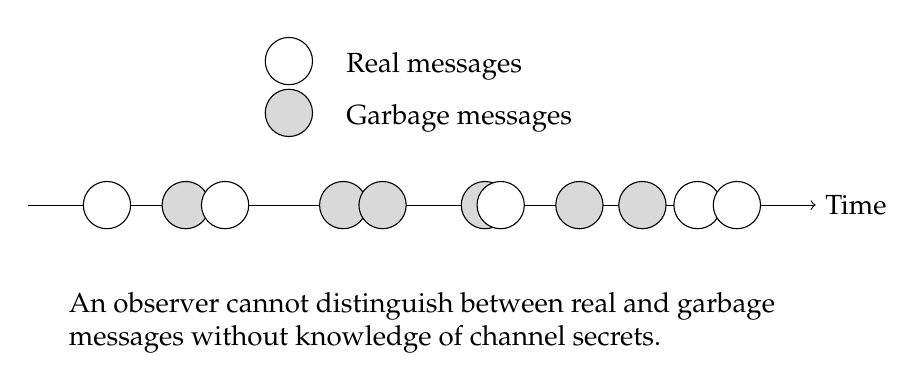
\begin{tikzpicture}[
        message/.style={circle,draw,fill=white,minimum size=6mm},
        garbage/.style={circle,draw,fill=gray!30,minimum size=6mm},
        description/.style={align=left}
    ]

    \draw[->] (0,0) -- (10,0) node[right] {Time};

    \node[message] at (1,0) {};
    \node[garbage] at (2,0) {};
    \node[message] at (2.5,0) {};
    \node[garbage] at (4,0) {};
    \node[garbage] at (4.5,0) {};
    \node[garbage] at (5.8,0) {};
    \node[message] at (6,0) {};
    \node[garbage] at (7,0) {};
    \node[garbage] at (7.8,0) {};
    \node[message] at (8.5,0) {};
    \node[message] at (9,0) {};

    \node[description] at (5,1.5) {
        \begin{tabular}{l l}
            \raisebox{-1ex}{\tikz\node[message] {};} & Real messages \\[0.5ex]
            \raisebox{-1ex}{\tikz\node[garbage] {};} & Garbage messages
        \end{tabular}
    };

    \node[description] at (5,-1.5) {
        An observer cannot distinguish between real and garbage\\
        messages without knowledge of channel secrets.
    };

    \end{tikzpicture}
    \caption{Real and garbage messages as seen by outside observers.}
    \label{fig:garbage_messages}
\end{figure}

\section{Payload size}\label{payload-size}

One of the most obvious pieces of metadata in an encrypted message is its size. A malicious actor observing network traffic over a long period of time may detect patterns in payload size which could allow the malicious actor to trace users across time.

The trivial solution to this is to enforce a regular payload size to which all messages must conform. This approaches a good solution to this problem, but it also introduces a number of drawbacks.

First, and most obviously, is that if the messages in question are much smaller than the standard size, it will result in a lot of wasted space on the message repository. If the message repository in question is a blockchain (a natural choice in many respects for this protocol), storage is quite expensive---many, many orders of magnitude beyond a commercial cloud provder like Amazon S3.\footnote{For instance, the Ethereum smart contract platform  charges 20,000 units of gas for a cold 256-bit storage write \parencite[][Appendix G]{wood_ethereum_2025}. At current gas prices of about 30 GWei (3E-8 Ether) \parencite{etherscanio_gastracker} and an Ether price of about \$3,400 \parencite{coingecko_ethereum_2025}, we calculate an approximate price of $3400 \si{\,USD\per Ether} \cdot 3.1 \times 10^{-8} \si{\,Ether\per gas} \cdot 20000 \si{\,gas\per slot} \cdot \frac{10^9 \si{\,bytes\per GB}}{32 \si{\,bytes\per slot}} = 6.6 \times 10^8 \si{\,USD\per GB}$: over \$600 million per gigabyte.}

\begin{figure}[h]
    \centering
    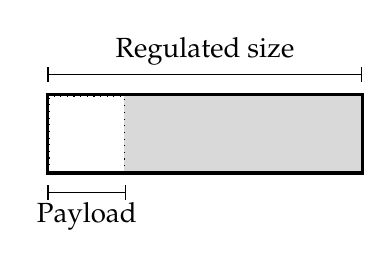
\begin{tikzpicture}[
        payload/.style={draw,dotted,fill=white,minimum width=9.5mm,minimum height=9.5mm},
        envelope/.style={draw,very thick,fill=gray!30,minimum width=40mm,minimum height=10mm}
    ]

    \node[envelope] (envelope) at (0,0) {};
    \node[payload] (payload) at (-1.5,0) {};

    \draw[|-|] (-2,0.75) -- (2,0.75) node[midway,above] {Regulated size};
    \draw[|-|] (-2,-0.75) -- (-1,-0.75) node[midway,below] {Payload};

    \end{tikzpicture}
    \caption{A smaller payload fits into a larger regulated-size envelope with padding.}
    \label{fig:payload_size}
\end{figure}

A converse problem of a regulated message size is for messages where the contents are longer than the regular size. Not only does this impose an overhead in the necessity of breaking up large messages to fit into the regular size, but the metadata that must be included in order for the receiver to properly parse the incoming messages may be cumbersome (or large).

However, even worse than the inefficiency problem are the potential privacy implications. Let us say, for example, that the regulated message size were 1 kibibyte (1024 bytes), but the user wished to send a 10-kibibyte message? Of course, the user must send at least 10 standard-sized messages to transfer the data outright. Unfortunately, if the user wishes to do this with any degree of efficiency, he must send those messages all in quick succession, even simultaneously. From the perspective of a party observing the user's network traffic, 10 simultaneous 1-kibibyte messages is not really much better than simply sending a single 10-kibibyte message.

\begin{figure}[h]
    \centering
    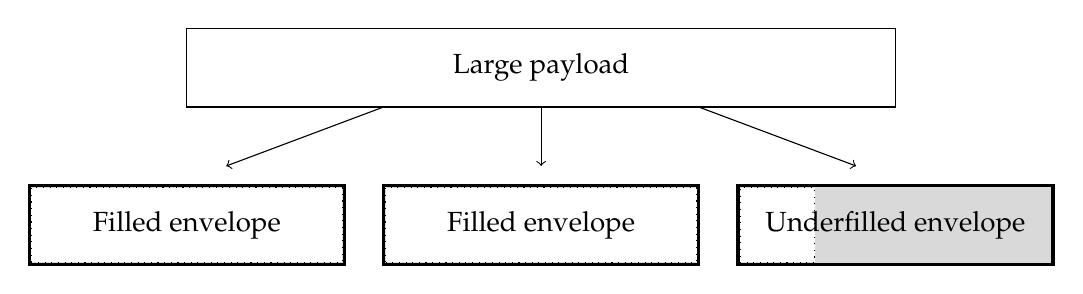
\begin{tikzpicture}[
        payload/.style={draw,fill=white,minimum width=90mm,minimum height=10mm},
        fullchunk/.style={draw,dotted,fill=white,minimum width=39.5mm,minimum height=9.5mm},
        chunk/.style={draw,dotted,fill=white,minimum width=9.5mm,minimum height=9.5mm},
        envelope/.style={draw,very thick,fill=gray!30,minimum width=40mm,minimum height=10mm}
    ]

    \node[payload] (payload) at (0,2) {Large payload};

    \draw[->] (-2,1.5) -- (-4,0.75);
    \draw[->] (0,1.5) -- (0,0.75);
    \draw[->] (2,1.5) -- (4,0.75);

    \node[envelope] (envelope1) at (-4.5,0) {};
    \node[fullchunk] (chunk1) at (-4.5,0) {Filled envelope};

    \node[envelope] (envelope2) at (0,0) {};
    \node[fullchunk] (chunk2) at (-0,0) {Filled envelope};

    \node[envelope] (envelope3) at (4.5,0) {};
    \node[chunk] (chunk3) at (3,0) {};
    \node[centered] at (4.5,0) {Underfilled envelope};

    \end{tikzpicture}
    \caption{A large payload split into multiple chunks, padded to fit regulated-size envelopes if necessary.}
    \label{fig:payload_chunks}
\end{figure}

Therefore, we expand this idea by introducing a range of regulated message sizes, e.g. 1-kb, 4-kb, 16-kb, 64-kb, to which each message must conform. It the responsibility of the client to choose the most effective set of message sizes to use when sending a particular message. The client could choose to send a 3-kb message in three 1-kb messages, or in a single 4-kb message, or in two 64-kb messages, depending on how the client implements a size-selection algorithm: optimizing for efficiency or masking?

Some kinds of messages may simply be too large to make practical use of a protocol with standardized message lengths, such as photographs and HD video. In this case, we recommend providing the actual contents over a separate medium (e.g. a centralized hosting provider), and simply transmitting the URI for the contents over the channel.

Combining payload size manipulation with garbage messaging provides us with a good set of tools to use to emit noise into the protocol amongst which genuine communications can hide.

\section{Proxies }\label{proxies}

Within the protocol itself we have already discussed many facets of metadata concealment. However, as other projects have noted in the past \parencite{erciccione_blog_2020, dingledine_tor_2004}, the network transport layer has the potential to leak metadata about participants as well.

Since network activity to this protocol is easily identifiable, it becomes necessary to implement some sort of hiding technique to conceal additional information such as origin and destination IP addresses. If an implementation of the protocol only includes such features as described previously, a malicious actor could observe network traffic to and from the message repository to discover that Sender Steve is a user of the protocol. Or, even worse, if the message repository is hosted on a cloud service that does not respect the privacy of its clients, or if it is controlled by, for example, a malicious state actor, the message repository itself could discover the origin IP address of Steve. The privacy of a message recipient could be discovered in a similar manner.

Although it is not strictly required by the protocol, it is convenient to use a blockchain as the message repository for this protocol. This creates an even more pertinent problem related to the transport layer in that blockchain activity is both permanent and public, meaning that interactions with the message repository are permanently visible to the entire blockchain. It is a trivial task to open up a blockchain explorer and retrieve historical activity between different accounts, pseudo-anonymous as they may be.

Therefore, it becomes necessary to introduce a further layer of separation between the actual user of the messaging protocol and the message repository. We propose the use of ``message proxies.''

A message proxy is a service that sits in-between the user of the protocol and the message repository. It is the responsibility of the proxy service to ingest messages sent by users and forward them to the repository, effectively eliminating metadata from the message that might reveal the identity of the user. From a network transport layer perspective, as well as from the perspective of the blockchain, messages would then be coming from the proxy service instead of directly from the user.

\begin{figure}[h]
    \centering
    \begin{tikzpicture}[
        entity/.style={circle,draw,solid,fill=white,minimum size=10mm},
        public/.style={rectangle,draw,solid,fill=white,minimum width=12mm,minimum height=8mm},
        service/.style={rectangle,draw=black,dotted,rounded corners=2em,minimum width=3cm,minimum height=2cm},
        proxy/.style={rectangle,draw=black,dotted,fill=gray!10,minimum width=6.5cm,minimum height=3.5cm}
    ]

    \node[proxy] (proxy) at (0,0) {
        \begin{tikzpicture}[
            every node/.style={
                draw=none,
                fill=none,
                rounded corners=0pt
            }
        ]
            \node[public] (payload) at (-2.5,-.5) {$(h,c)$};
            \node[public] (replacement) at (-2.5,.5) {$c'$};
            \node[public] (newpayload) at (1,0) {$(h,c')$};

            \draw[->,solid] (payload) -- (newpayload);
            \draw[->,solid] (replacement) -- (newpayload);
        \end{tikzpicture}
    };

    \node at ($(proxy.north east)+(-1,-.75)$) {Proxy};

    \node[entity] (user) at ($(payload.west)+(-1.5,0)$) {User};
    \node[service,align=center] (repo) at ($(newpayload.east)+(4,0)$) {Message\\Repository};

    \draw[->,solid] (user) -- ($(payload.west)+(.75,0)$);

    \draw[->,solid] ($(newpayload.east)+(.75,0)$) -- (repo);

    \end{tikzpicture}
    \caption{A malicious proxy manipulates message contents while preserving sequence hash.}
    \label{fig:proxy_manipulation}
\end{figure}

Of course, this merely kicks the can down the road, per se, since now the trust issues associated with a compromised message repository are now conferred upon a compromised proxy service.

Furthermore, while we have previously assumed that a user may interface and transact directly and, most importantly, \emph{immediately}, with a blockchain, that is not remotely true. In fact, the proxy service merely makes the problem more obvious: that a man-in-the-middle may intercept a message from a genuine user, replace the message payload with anything else, and submit the maliciously-constructed message to the blockchain before the genuine one has a chance to make it, thereby ``sniping'' a real sequence hash. If the proxy server is itself untrustworthy, it is even easier to steal sequence hashes from authentic payloads and never forward said payloads to the message repository in the first place.

\subsection{Ensuring proxy honesty}\label{ensuring-proxy-honesty}

Therefore, it becomes necessary to enforce some sort of safeguard that prevents a malicious actor from stealing genuine sequence hashes from authentic payloads while they are in flight. Until this point in the description of the protocol, the message repository has been a low-complexity service, merely enforcing that values associated with stored keys may not be overwritten.

Now we introduce another criterion: a proof that the value to be stored under a key actually \emph{belongs} in that storage slot. Since the message repository does not necessarily impose authentication measures, each proof must be self-contained. This use-case dictates that the proof must show that some property of the payload links it to the preimage of the sequence hash. Recall that the sequence hash is composed of, among other things, the shared secret among channel members. At first glance, including some sort of digital signature seems to accomplish a great deal of our goal, but closer inspection reveals that a digital signature must be verified against a known public key, the use of which would compromise the identities of participants and/or link multiple messages from the same channel together, eliminating many of the protocol's desirable qualities.

Therefore, instead of relying on traditional signature verification, we turn to a new player on the modern cryptographic stage: zero-knowledge proofs (ZKPs). A ZKP proves to a verifier that a prover is in possession of some knowledge without revealing to the verifier anything about that knowledge. \parencite{goldwasser_knowledge_1985}

There are many different systems that can be used to generate zero-knowledge proofs, but the specifics of choosing a proof system is well beyond the scope of this paper. Rather than overconstrain this protocol description with a specific implementation, we recommend optimizing for proof verification efficiency when choosing a system, since the use-case involves verifying many small proofs.

In our case, Sender Steve wants to prove that he knows the secret channel identifier $i_{\{S,R\}}$ necessary to both produce the sequence hash and encrypt the accompanying ciphertext without revealing it to the proxy, the message repository, or anyone with read access to the message repository. The ZKP circuit to prove such a statement looks something like the following code listing.

\begin{minted}{python}
def verify(
    public image,
    public ciphertext,
    private key,
    private preimage_rest,
    private message):

    preimage = concat(key, preimage_rest)

    assert digest(preimage) == image
    assert encrypt(message, key) == ciphertext
\end{minted}

Sender Steve will be responsible for generating a proof by constructing a set of public and private inputs which satisfy the circuit. In the case of the circuit pseudocode in the listing above, Steve would be responsible for providing public inputs of the sequence hash $h_{\{S,R\}}^n$ and ciphertext $c^n$, as well as the private inputs of the shared secret $k_{\{S,R\}}$, the rest of the information required to compute the sequence hash (such as the message index $n$), and the cleartext of the message. Since these latter items are part of the private inputs, they will not be revealed in the proof that is generated.

Upon constructing this proof, Sender Steve packages the three items---sequence hash, ciphertext, and proof: $(h_{\{S,R\}}^n, c^n, \pi^n)$---all together and sends them off to the message distributor (either directly to the message repository, or to the proxy if that service is in effect).

When the message repository receives this triplet, it first verifies the proof with the well-known circuit and the provided sequence hash and ciphertext. If the proof can be successfully verified, only then does the message repository write the ciphertext into its key-value store.

If a malicious third-party, Malicious Max, intercepted the triple and attempted to replace the ciphertext payload with one of his own design, he would not be able to also generate a ZKP proving foreknowledge of the private inputs that Steve knows: in particular, the shared secret. Thus Max, regardless of whether he is merely a man-in-the-middle or the veritable operator of a proxy, is unable to ``snipe'' sequence hashes from genuine payloads.

\section{Dandelion-style routing}\label{dandelion-style-routing}

Let us suppose there is an Observer Ollie of the network, including the message repository, the proxies, and the message sender. Ollie is able to observe the activity between each of the network participants, but not able to see the internal memory or computational activities of any of them. Because the message repository is publicly readable by anyone, Ollie is able to monitor the message repository for new messages. Therefore, Ollie can detect when a message sent by Steve appears on the message repository, and can therefore learn the sequence hash of a message known to have been sent by Steve. Continuing to monitor the network activity of all participants could further reveal to Ollie the identity of the message receiver Robin. (However, if we assume impenetrably encrypted network communication tunnels, this step may require additional techniques beyond simple surveillance.)

\begin{figure}[h]
    \centering
    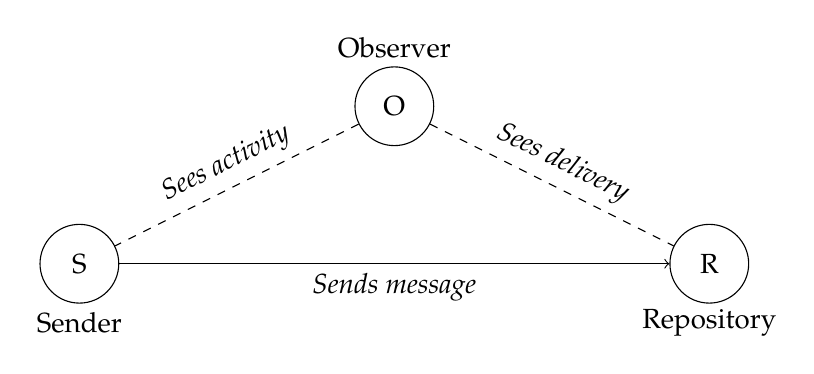
\begin{tikzpicture}[
        participant/.style={circle,draw,fill=white,minimum size=10mm},
        description/.style={align=left}
    ]

    \node[participant] (steve) at (-4,0) {S};
    \node[description] at (-4,-0.75) {Sender};

    \node[participant] (repository) at (4,0) {R};
    \node[description] at (4,-0.75) {Repository};

    \node[participant] (ollie) at (0,2) {O};
    \node[description] at (0,2.75) {Observer};

    \draw[->] (steve) -- (repository)
        node[midway,below] {\textit{Sends message}};

    \draw[dashed] (ollie) -- (steve)
        node[midway,above,sloped] {\textit{Sees activity}};
    \draw[dashed] (ollie) -- (repository)
        node[midway,above,sloped] {\textit{Sees delivery}};

    \end{tikzpicture}
    \caption{Network observer monitoring message sender and repository.}
    \label{fig:observer}
\end{figure}

Therefore, the protocol is in need of a feature to break (or at least obfuscate) the network activity link between a sender distributing a message payload and that message payload appearing on the message repository.

When attempting to conceal the activity of network participants, many projects have adopted similar measures to that which we propose here: that of passing messages amongst multiple peers before delivering it to its final destination, and concealing the true origin in the process. Most prominently among such projects may be The Onion Router, more commonly known as Tor. Put simply, a user chooses a path through his peers and wraps his request in multiple layers of encryption which each subsequent peer in the path is able to decrypt. A similar proposal was made for the Bitcoin network \parencite{venkatakrishnan_dandelion_2017}, and a variation of it \parencite{fanti_dandelion_2018} was adopted by Monero in 2020 \parencite{erciccione_blog_2020}.

Introducing this feature to our protocol requires the increase from a single proxy service to multiple, unaffiliated proxy services. ``Unaffiliated'' is an important qualifier: the proxy network members (relays) must have sufficiently disparate interests and controlling influences to ensure that they are not incentivized to cooperate with each other to reveal the payload paths throughout the network. \parencite{douceur_sybil_2002, paganini_attacks_2014}

This feature is not without its downsides: not only does it add nontrivial amounts of complexity to the development and maintenance of the protocol---properly implementing the Dandelion-style routing is a significant up-front cost, and maintaining a large, decentralized network of routing proxies is a significant maintenance cost---it also adds a noticeable amount of latency to the message sending process. From a privacy perspective, this is not entirely bad, since high and highly-variable latency between dispatch and receipt by the message repository can reduce the correlations in network activity timings, but it has an exclusively negative impact on the user-friendliness of the protocol.

Even assuming an honest network of relays, timing attacks are a further deanonymization technique. \parencite{defconconference_def_2013} Because each member of the proxy network should be publicly accessible, this allows for sidechannel deanonymization attacks: though the technique presented by Evans and Grothoff relies on a malicious JavaScript injection to ``phone home,'' simple observation of the message sender along with the message repository over a long enough period could serve the same purpose of latency measurement.

\section{Message notifications}\label{message-notifications}

The life of a message receiver is rather drab and repetitive. Receiver Robin has a simple responsibility: check the message repository to see if the next sequence hash exists. It does exist? Great, download the message! It does not exist? Go back and check again, repeating until it shows up. Robin simply plies the message repository with ``message notification'' requests until he receives the message (then he starts looking for the next message) or he goes offline.

Unfortunately, upon closer examination, some issues with this model become apparent. In the same vein as the previous section, wherein we addressed the potential for network activity analysis to deanonymize message senders, similar analysis can serve to deanonymize receivers. However, it is arguably slightly more risky for the receivers, because they check for the same sequence hash multiple times, meaning that a network observer need only be observing the network for long enough to witness a single message notification request. (Note that in the case of a blockchain environment, an RPC node operator could easily be this ``network activity observer,'' for whom observation is significantly easier to perform than a traditional man-in-the-middle sniff.) The knowledge that a user searching for a particular (as of yet undelivered) message is likely to inquire about the sequence hash multiple times again in the future enables attackers to execute more targeted deanonymization attempts.

Thus, the first privacy-enhancing option available to the message receiver is to adopt the same dandelion-style network that the message senders are using, except to use it for sending message notification requests instead of for transmitting message payloads. While this would conceal the origin of the requester on a per-request basis, it is not as clean of a solution as it is in the case of the message sender: a network observer can still detect when a user (that is, for example, via activity originating from an IP address) joins the network, and if requests for a certain sequence hash are made in elevated frequency when a certain user is also active on the network, it may not be necessary to trace the exact route of a request back to its origin to establish with reasonably high confidence that this certain user is interested in this certain sequence hash.

Malicious network observations of message notification requests reveal (potentially) unused-yet-valid sequence hashes to attackers. If the zero-knowledge proof extension is not implemented, then this system requires assuming the trustworthiness of the message repository and all handlers of unencrypted (that is, by a TLS tunnel or similar) payload data between the message repository and the message receiver to not ``snipe'' the valid sequence hash and insert it with a malicious or garbage payload before the real message has a chance to land. But, the goal of this protocol is to minimize the trust users must have in these entities. With the zero-knowledge proof extension, the risk of sequence hash ``sniping'' is reduced, but the risk of correlating user activity with particular sequence hash read requests is not. Thus, we understand that the protocol is in need of a mechanism for allowing message receivers to check for the presence of a particular sequence hash without divulging to anyone on the network which sequence hash it is.

Furthermore, it is unlikely that a single receiver will only be interested in checking for the existence of a single message. Rather, a single user of the protocol is probably going to be listening for the existence of a multitude of different messages. This would impose a serious bandwidth requirement on even light users of the protocol. The reference implementation of this protocol uses a few types of control messages (messages containing instructions to the application, rather than directly human-readable plain text) which might be transmitted across designated channels. This practice in combination with a user who is only communicating with a few different users and/or groups already imposes a heavy burden of network usage on the user if they wish for their communications to be even vaguely real-time.

Therefore, while using the dandelion-style proxy network for checking for individual sequence hash notifications is certainly an improvement over direct requesting, there is a fundamental disconnect in the approach: Robin wishes the message repository to tell him whether specific sequence hashes exist without identifying those hashes.

\subsection{Message notification filters}\label{message-notification-filters}

To solve this conundrum, we introduce a sequence hash Bloom filter. \parencite{bloom_space_1970} Upon writing a message to its storage, the message repository also inserts\footnote{It is not necessary that the Bloom filter is constructed immediately. It could, for example, be constructed on-demand if the cost of storage on the message repository is higher than that of compute.} the sequence hash into a Bloom filter. In order to maintain an acceptable false-positive rate, the current ``message notification filter'' is archived at regular intervals. Archived and current filters can be requested by users. This structure allows a message receiver awaiting the delivery of one or more sequence hashes to download a single payload within which he can check for the presence of any number of sequence hashes. If the user has not synchronized with the network recently, he can download archived filters to the same effect.

In the case that the message repository generates the message notification filters on-demand, the message repository should \emph{not} allow clients to specify a custom timeframe of sequence hashes to include, due to potential metadata leakage pertaining to when the client in question last synchronized with the network.

While this approach succeeds in concealing the sequence hashes for which a message receiver is intent on listening, it increases network load and worsens latency. Whereas a simple, direct query to the message repository would be nearly negligible in terms of network load---a request object containing merely a sequence hash and response merely a boolean---the size of a Bloom filter scales linearly with the maximum number of insertions given a false-positive rate, where the maximum number of insertions is the maximum number of messages that the message repository can process before archiving the current message notification filter. Where $p$ is the desired false-positive rate, the number of bits required per element $b$ is given by:

$$ b = \frac { \ln \left( \frac{1}{p} \right) }
  {\ln ^2 \left( 2 \right) } $$

Meaning that a modest 1\% false-positive rate commands about 9.6 bits per sequence hash. \parencite{cortesi_3_2010}

The apples-to-apples comparison with authenticated (albeit end-to-end encrypted) server messaging platforms is quite bleak, as they have no such scaling limitation. However, compared with other public ledger/private activity-style platforms which may require downloading and scanning the entirety of the ledger \parencite{monerohow_low_level_2024}, the expense of \textasciitilde10 bits per sequence hash is comparatively low.

\subsection{Garbage message requests}\label{garbage-message-requests}

While the Bloom filter approach does have the advantage of providing a quasi-offline means of checking whether a particular set of sequence hashes are reasonably likely to have been posted to the message repository, the inextractibility of elements contained within the Bloom filter actually prevent a mirror strategy to the \hyperref[garbage-messages]{``garbage messages''} suggested previously.

If Receiver Robin is concerned that requesting a certain extant sequence hash may link his identity to that of Sender Steve, Robin might consider sending bogus requests for other extant sequence hashes to conceal the genuine request amongst false ones. However, if the primary means by which Robin learns about the state of sequence hashes in the message repository is via the message notification filter, there is not a reasonable way for Robin to be able to know other extant sequence hashes without constructing them himself (implying knowledge of the secrets necessary to calculate them) or plainly asking for them (implicitly confessing a lack of knowledge of the secrets necessary to calculate them).

When sending messages, a user also sends out some garbage messages as noise. Assuming a network Observer Ollie who is attempting to deanonymize users based on inter-participant network and message repository activity, Ollie can observe certain messages that never get read. Ollie, having knowledge of the protocol, realizes that these messages are likely to be garbage messages, and therefore excludes them from his network analysis after some time.

Therefore, we make the following recommendation.

When this user sends out some garbage messages, the user retains the sequence hashes\footnote{Or simply the minimum information necessary to reproduce them.}, additionally sending out garbage message \emph{requests} later on to imitate a receiver coming on-line and detecting the delivery of an expected sequence hash. It should be noted that the delay between sending and ``receiving'' a garbage message should be highly variable, with some garbage messages not getting ``received'' at all.

\chapter{Implementation}\label{Implementation}

\href{https://github.com/encody/near-private-data}{A reference implementation for this paper is available.}

The proof-of-concept is a simple command-line application that allows for $1 \leftrightarrow 1$ messaging between two parties. The proof of concept is written in Rust, and uses the \href{https://github.com/dalek-cryptography}{\emph{Dalek} libraries} for cryptographic primitives, as well as \href{https://github.com/RustCrypto/AEADs/tree/master/chacha20poly1305}{\emph{ChaCha20-Poly1305}} for encryption.

Even without enabling many of the privacy-enhancing features, the simple application struggles to approach real-time communications, with regular
latencies of 1-3 seconds.

\chapter{Prior Art}

\label{PriorArt}

\section{BitMessage}\label{bitmessage}

BitMessage \parencite{warren_bitmessage_2012} is a Bitcoin-inspired message transfer protocol. We highlight some notable differences in the functionality of the BitMessage protocol and our proposal.

\begin{enumerate}
\item Sending a message over the BitMessage network requires a proof-of-work, guaranteeing a latency floor in the protocol. Our protocol only requires such proofs as the underlying infrastructure, with \hyperref[ensuring-proxy-honesty]{an optional extension for zero-knowledge proofs}.
\item All users connected to the BitMessage network receive all messages. Users of our protocol know beforehand which messages are intended for them and can retrieve only those in a privacy-preserving fashion. There is \hyperref[message-notifications]{an optional extension for message notifications} that incurs an \(O(n)\) space cost on users where \(n\) is the number of messages sent to the message repository.
\item Broadcast messages may be sent on the BitMessage network, but they are visible to all users of the network who wish to view them. Our protocol supports arbitrarily large broadcast groups with \(O(1)\) sending cost, simply by sharing a new channel key.
\item Messages on the BitMessage network are deleted after a period of two days. Our protocol uses an indelible append-only ledger (i.e.~blockchain) from which messages cannot be erased.
\end{enumerate}

%-----------------------------------
%	SUBSECTION 1
%-----------------------------------
\section{Signal Double-Ratchet}\label{signal-double-ratchet}

Considered by many to be the gold standard in modern encrypted messaging, the Signal Double-Ratchet protocol \parencite{perrin_double_2016} implements a foreboding trifecta of privacy properties: resilience, forward security, and break-in security. The sequence hashes from our protocol exhibit the first of these properties.

One of the issues experienced by many protocols in this sector is that while the messaging protocol may be clearly cryptographically and mathematically sound, correctly implementing such fancy techniques as deniability, if transcripts of the conversation are revealed, those hard mathematical evidences do very little to effectively recuse a conversant from a conversation. This has led some protocols to discount such techniques entirely. \parencite{jefferys_session_2020}

The experimental techniques presented in this paper do not endeavor to implement complete deniability in the traditional sense, due in large part to the nature of the invariants required by the infrastructure upon which they depend. That is to say, it would violate the fundamental contract of an ``append-only public ledger'' if two plausible transcripts could be provided that purport a different sequences of appends.

Rather, we take a different approach. One of the problems with simply implementing something like the Signal Double-Ratchet algorithm is that while it hides the \emph{content} of the messages between conversants Alice and Bob, it does not hide the fact that Alice and Bob are (1) conversing, or (2) conversing with each other. The flexible channels protocol in itself does attempt to conceal this information. However, it should be duly noted that the protocol as presented assumes the existence of some sort of public-key infrastructure (PKI). PKIs are usually publicly-accessible, so the presence of a user's public key in the PKI could belie their usage of the protocol. This issue can be mitigated somewhat by (1) using a PKI that has sufficient quantity of users for a diverse variety of applications, or (2) not using a public PKI, and instead manually facilitating public key exchanges (e.g. by meeting in person, scanning QR codes, etc.).

\chapter{Conclusion}\label{Conclusion}

We present Flexible Channels, an experimental foray into encrypted messaging over public, append-only message repositories such as blockchains. The key insights of this research are the channel and sequence hash constructions which allow for privacy-friendly messaging across public message repositories using simple, traditional cryptography.

We explore a number of benefits of this infrastructure, including easy cross-device message synchronization, uncensorability, and $O(1)$ broadcast messaging.

However, the protocol as described and implemented immediately suffers severe performance impairments that preclude its adoption. Regardless of its performance, the infrastructure does not provide significant improvements over existing practices of end-to-end encryption through authenticated servers, and the privacy implications of permanently etching ostensibly secret messaging history onto an inextirpable public record encrypted merely by means which are considered secure by the standards of today cannot be understated. The protocol as described does not enforce any sort of forward secrecy, although it is flexible enough to allow e.g. key rotation within channels, so the design does not preclude the implementation of this privacy-critical feature.

Therefore, while we cannot yet recommend using this protocol in non-experimental contexts, we are pleased to submit this novel combination of techniques for critique and edification.

Possible future applications of similar technology could become feasible in environments with a forcing need for public auditability juxtaposed with privacy (e.g. government operations or highly-regulated industries).


%----------------------------------------------------------------------------------------
%	BIBLIOGRAPHY
%----------------------------------------------------------------------------------------

\printbibliography[heading=bibintoc]

%----------------------------------------------------------------------------------------
%	THESIS CONTENT - APPENDICES
%----------------------------------------------------------------------------------------

\appendix % Cue to tell LaTeX that the following "chapters" are Appendices

% Include the appendices of the thesis as separate files from the Appendices folder
% Uncomment the lines as you write the Appendices

% % Appendix A

\chapter{Frequently Asked Questions} % Main appendix title

\label{AppendixA} % For referencing this appendix elsewhere, use \ref{AppendixA}

\section{How do I change the colors of links?}

The color of links can be changed to your liking using:

{\small\verb!\hypersetup{urlcolor=red}!}, or

{\small\verb!\hypersetup{citecolor=green}!}, or

{\small\verb!\hypersetup{allcolor=blue}!}.

\noindent If you want to completely hide the links, you can use:

{\small\verb!\hypersetup{allcolors=.}!}, or even better: 

{\small\verb!\hypersetup{hidelinks}!}.

\noindent If you want to have obvious links in the PDF but not the printed text, use:

{\small\verb!\hypersetup{colorlinks=false}!}.

%\include{Appendices/AppendixB}
%\include{Appendices/AppendixC}

%----------------------------------------------------------------------------------------

\end{document}
